\documentclass[11pt,parskip=full]{scrartcl}%article}
%\setlength{\parskip}{1em}

%%%%%%%%%%%%%%%%%%%%%%
%% PACKAGE INCLUDES %%
%%%%%%%%%%%%%%%%%%%%%%

\usepackage{array}           % For defining \newcolumntype.
\usepackage{amsmath}
\usepackage{amssymb}
\usepackage{amsthm}          % Provides 'proof' environment.
\usepackage[english]{babel}  % For defining 'theorem/corollary/lemma' environments.
\usepackage{bm}              % Provides bold \pi
\usepackage{booktabs}
\usepackage{hyperref}
\usepackage{textcomp}
\usepackage{gensymb}         % Enables \degree command for °C.
\usepackage{todonotes}
\usepackage{subfig}
\usepackage{enumitem}
\usepackage{graphicx}
\usepackage{listings}


%%%%%%%%%%%%%%%%%
%% STYLE SETUP %%
%%%%%%%%%%%%%%%%%

% Define some custom colors.
\definecolor{mylinkcolor}{RGB}{000, 114, 166}
\definecolor{mycitecolor}{RGB}{255, 154, 071}
\definecolor{myurlcolor}{RGB}{000, 114, 166}

% Set itemize format.
\setitemize{noitemsep,topsep=-5pt,parsep=5pt,partopsep=0pt}

% Define column types that allow fixed width params.
\newcolumntype{L}[1]{>{\raggedright\let\newline\\\arraybackslash\hspace{0pt}}m{#1}}
\newcolumntype{C}[1]{>{\centering\let\newline\\\arraybackslash\hspace{0pt}}m{#1}}
\newcolumntype{R}[1]{>{\raggedleft\let\newline\\\arraybackslash\hspace{0pt}}m{#1}}

% Color setup for hyperlinks/references/citations/urls.
\hypersetup{
    colorlinks,
    linkcolor={mylinkcolor},
    citecolor={mycitecolor},
    urlcolor={myurlcolor}
}

% Specify hyphenation of words on line break.
\hyphenation{Figure Table Chapter Section}



%%%%%%%%%%%%
%% MACROS %%
%%%%%%%%%%%%

% Set default font family to sans-serif.
\renewcommand*{\familydefault}{\sfdefault}
\newcommand{\Tau}{\mathrm{T}}

\newcommand*{\ie}{i.e., }
\newcommand*{\eg}{e.g., }
\newcommand*{\wrt}{w.r.t. }

\newcommand*{\tokens}{\mathcal{T}}          % Set of tokens.
\newcommand*{\orders}{\mathcal{O}}          % Set of orders.
\newcommand*{\itokens}{\mathcal{I}^t}       % Set of token indices.
\newcommand*{\itokenpairs}{\mathcal{I}^p}   % Set of token index pairs.
\newcommand*{\iorders}{\mathcal{I}^o}       % Set of order indices.
\newcommand*{\ibuyorders}{\mathcal{I}^b}    % Set of buy order indices.
\newcommand*{\isellorders}{\mathcal{I}^s}   % Set of sell order indices.

% Macros for references etc.
\newcommand*{\figref}[1]{\hyperref[{#1}]{Figure~\ref*{#1}}}
\newcommand*{\tabref}[1]{\hyperref[{#1}]{Table~\ref*{#1}}}
\newcommand*{\secref}[1]{\hyperref[{#1}]{Section~\ref*{#1}}}
\newcommand*{\subsecref}[1]{\hyperref[{#1}]{Section~\ref*{#1}}}
\newcommand*{\thmref}[1]{\hyperref[{#1}]{Theorem~\ref*{#1}}}
\newcommand*{\crlref}[1]{\hyperref[{#1}]{Corollary~\ref*{#1}}}
\newcommand*{\lemref}[1]{\hyperref[{#1}]{Lemma~\ref*{#1}}}

% Macros for theorems|corollaries|lemmas.
\newtheorem{theorem}{Theorem}[section]
\newtheorem{corollary}{Corollary}[theorem]
\newtheorem{lemma}[theorem]{Lemma}


%Notational abbreviations

\def\pO{\mathcal{O}}
\def\ra{\rightarrow}

\newcommand*{\erc}{ERC20 } 

%%%%%%%%%%%%%%
%% DOCUMENT %%
%%%%%%%%%%%%%%

\title{
  Multi-token Batch Auctions with Uniform Clearing Prices on Plasma\\
  - \\
  \Large Specification For Implementation}
\author{Gnosis}

\date{\today}



\begin{document}

\maketitle


\begin{abstract}

This document outlines a formal specification of a batch auction exchange of ERC20 tokens using the plasma technologies. The batch auction mechanism will enable the execution of ring trades between different tokens. Plasma technologies will provide the same security for users as if the tokens were held in the ethereum blockchain. But gas costs will be significantly reduced due to the off-chain nature of the exchange mechanism. It is recommended for the reader to familiarize themselves with Plasma\cite{plasma}, Plasma MVP\cite{MVP}, snarks\cite{snarks} and batch auctions\cite{batch} before reading this spec.

\end{abstract}

\tableofcontents

\newpage
\section{Introduction}
\label{sec:introduction}

\paragraph{Multi-batch auctions with uniform clearing prices}

This specification outlines a trading mechanism between several \erc tokens. Each batch accepts orders to buy any \erc token with any other \erc token for a maximal specified limit price. All orders are collected over some time interval and then an \emph{uniform clearing price} over all token pairs is calculated. 
For a list of $k$ trading tokens denoted by $\Tau$ with clearing prices $\{p_{A|B}\}$, we call the set of prices $\{p_{A|B}| A,B \in \Tau \}$ an uniform clearing price, if
\begin{align} \label{eq:arbitrage_freeness}
  p_{A|B} \cdot p_{B|C} &= p_{A|C}\\
  p_{A|B} &= p_{B|A}^{-1}
\end{align}

Finding the uniform clearing prices, which also maximize trading volume and "traders welfare" is a complicated task. The paper []\todo{cite Tom?} describes a mechanism in detail. Uniform clearing prices are beneficial for any trader since they are arbitrage-free and ensure good liquidity via built-in ring trades. For the purpose of this document, it is assumed that these uniform clearing prices for a multi-batch auction can be efficiently determined. \newline
The multi-token batch mechanism is secured against front-running\footnote{front-running is a form of attack ...} by allowing users to submit encrypted orders into the batch auction. Only after the batch has closed will the orders be revealed and then the prices can be computed. 


\paragraph{Plasma minimal viable product}

This paper describes the specification for porting this auction mechanism onto a plasma chain. Plasma chains are a second layer scaling solution for blockchains which allow processing a much higher volume of transactions as the underlying blockchain (a.k.a. \emph{main chain}) with the same security guarantees. This is the main motivation for implementing such mechanism on a plasma chain as it will result in significantly trade costs with respect to gas fees. Although plasma chains have great advantages\todo{such as}, they also come with burdens in terms of usability and complexity.

\paragraph{The trade-flow of a batch auction}  

The batch auction exchange is built on a plasma chain operated by a single entity on top of a root-chain (Ethereum). A single batch auction consists of several phases;
\begin{itemize}
\item[(i)] Encryption Key generation, 
\item[(ii)] Order Collection, 
\item[(iii)] Double Signing, 
\item[(iv)] Batch Price Calculation, 
\item[(v)] Batch Challenging and 
\item[(vi)] Order Executions. 
\end{itemize}
In brief, a batch will proceed as follows: Users will post encrypted orders to the plasma operator, who will then bundle these orders and commit them by posting a single order-block on the plasma chain. Each client will have to validate all orders in the committed hash and only once they validate the orders, they may double sign their orders to participate in the current batch. The participation acknowledgment will be compactly represented using a crypto-economic signature aggregation schema. With this construction many data-unavailability problems will be avoided because the orders can be represented on the main-chain using only a bitmap.
Once the bitmap is seen by many parties on the plasma chain, the private key for decrypting the orders will be generated using distributed key generation (DKG). Finally, all the data is available to calculate correct prices from the orders and the batch can be settled. 

\newpage

\section{Detailed specification overview}
\subsection{Setup description}

\subsubsection{Definitions}

%Let us start of with writing down some very basic definitions, which we will use throughout this paper.
In our (batch) auctions all trading will occur between a fixed set, $\Tau = \{\tau_i\}_{i=1}^n$, of $n$ \erc tokens. The collection of orders for which token $i$ is being sold in exchange for token $j$ will be denoted by $\pO_{i\ra j}$. 

After an auction has closed uniform clearing prices have been determined, the price matrix can be represented as an $n\times n$ a matrix 
\[P = \{p_{ij}| \tau_i, \tau_j \in \Tau \}.\]
For any order $\sigma \in \pO_{i\ra j}$ we define $\nu_p(\sigma)$ as the volume of an order denominated in token $\tau_i$ at clearing prices $p$.

\subsubsection{Plasma chain setup}
We are following the description of the Plasma Minimal Viable Product, as it is described in \cite{MVP}. This means all assets are represented in the plasma chain as unspent transaction outputs (utxo). These utxos can be transferred to a new owner by making a transaction, waiting for its inclusion into the plasma chain, validating the chain, waiting for the plasma block to be submitted to the main-chain and then, sending a double-sign message to the receiver. 

Any utxo may be exited at any time, by providing a Merkle proof of the receiving transaction. However, if the exit is not valid, then it will be canceled via a challenge process.
Note that the plasma implementation will require users to be online and validate the chain's state at least once a week\todo{Why is this?}. If one seeks to participate in an auction, they would need to be online to broadcast their order, double sign and to receive/validate the order-output block message.




\subsection{The trade flow}
\label{subsec:data}

In the following section we will describe the general tradeflow through all its phases: Encryption Key generation, Order Collection, Double signing, Batch Price Calculation, Batch Challenging and Order Executions.


\begin{figure}
\centering
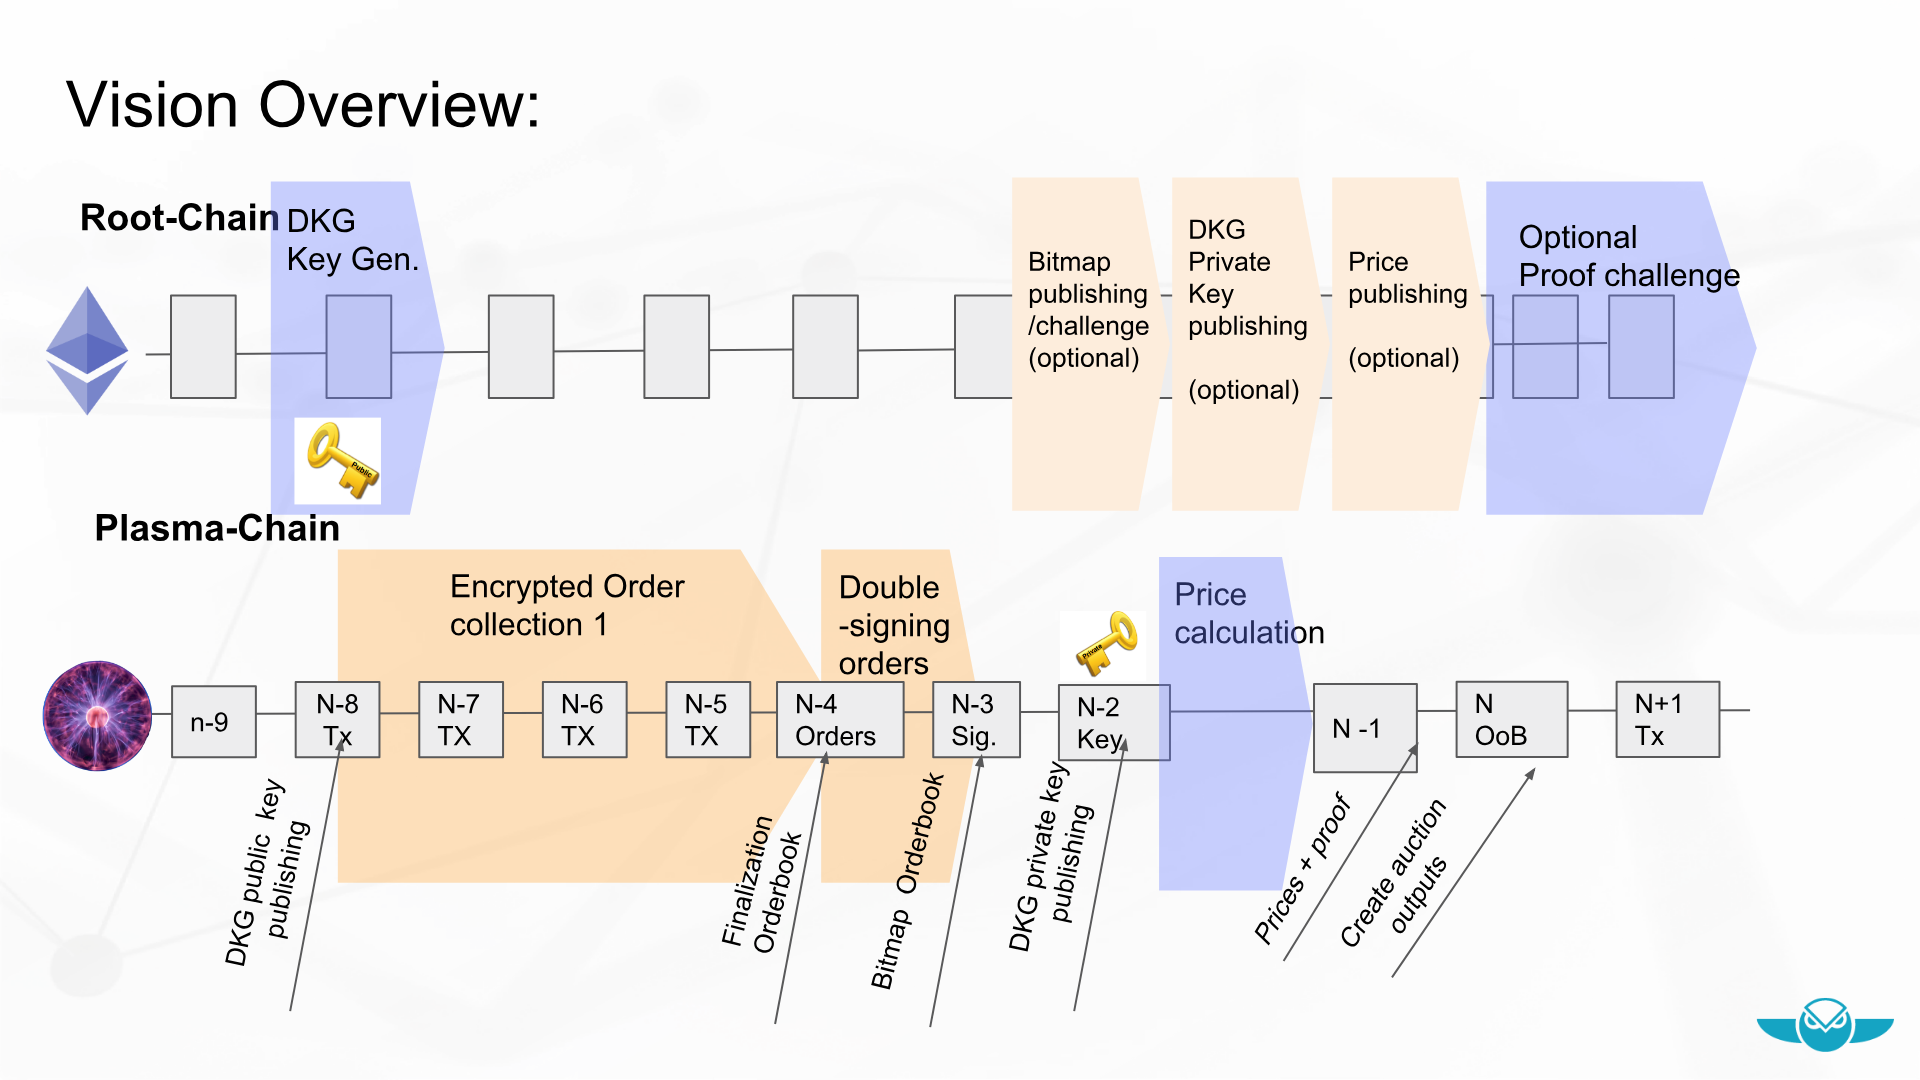
\includegraphics[width=\textwidth]{overview_tradeflow.png}
\end{figure}



\subsubsection{Encryption Key Generation}
All orders will be encrypted with a public key generated by the Distributed Key Generation (DKG) algorithm \cite{DKG}. A predefined number of bonded participants will be part of the DKG algorithm.  By exchanging special messages and withholding others, they will generate a new public key, for which the private decryption key is not known to any single participant. Only later, after the closing of the batch auction, the participants are asked to publish their private messages for the generation of the private key for the decryption of the orders. If a predefined threshold of participation is met, then this will allow anyone to generate the private key. If the participants publish their key previous to the closing of the batch and its documentation on the root-chain, the protocol will allow to slash them. Using this approach, we will have encrypted orders, unless a big portion of bonded DKG participants is malicious.

The DKG algorithm generates a public key represented as an elliptic point $aG\label{public key}$, for a generator G and a secret $a\in \mathbb{N}$. This public key can then be used to encrypt messages via the ECIES \cite{ECIES}. Each trader calculates $bG \label{salt}$ for a random natural number b and publishes this number in his order. Then he calculates: $baG$ and determines from this number the symmetric key pair for encrypting his order. A good symmetric encryption mechanism for our purpose would be Knudsen-Nyberg cipher \cite{cipher}. Later, once $a$ is public, we can decrypt the orders by calculating $abG$, which equals $baG$.


\subsubsection{Order collection}
\label{orderblock}
Once the public key for the encryption process is available, every trader can submit orders. In the plasma chain, all assets of the ERC20 tokens are represented with unspent transaction outputs (utxo). An order will refer to a utxo of an ERC20 token A and this utxo will be exchanged for the specified token B for a price below or equal to the given, encrypted limit price.
\begin{lstlisting}
Order[   UTXO TokenA,
	Encrypted(limit price),
	address TokenB,
	encryption salt,
	Other data: references and signatures]
\end{lstlisting} 
The encryption salt is the elliptic point used for encryption:  $bG$ (cp. \ref{salt}).
All orders will be collected and board-casted in one block per auction, the order-block. All orders included in this order-block will be able to participate in the next auction. Theoretically, the chain operator can censor orders, but since they are encrypted, he does not know what he is censoring. Sometimes the operator needs to censor some orders since, in a single batch, there shouldn't be more than $2^{16}$ orders. \newline
If users want to cancel their order, they should spend their utxo referred in their order.

\subsubsection{Double signing process}
Once the block with the orders is published and the Merkleroot hash is submitted in the root-chain, every participant in the batch auction needs to validate this new block and the complete chain. Once they commit that their order should be included in the next batch, they will all be able to withdraw their order funds only with the priority of this order-block. (This will be explained in detail here: \ref{exitRules}).
If participants validated the whole chain, they can send the operator the double signing message to signal that they want to participate.
\begin{lstlisting}
DoubleSign      [OrderHash,
		OrderbookBlockHash,
		BatchIndex,
		Signature]
\end{lstlisting}
The operator collects all these double signed messages and constructs a bitmap, in order to generate a crypto-economic signature aggregation (cp. \cite{sig}). If the operator gets a double signed message for the order at the i-th place in the block, then the operator puts a 1 into the bitmap at the i-th place. Otherwise, he puts a 0 in there. Next, the operator publishes the bitmap and all signature messages in a next plasma block. If the bitmap is not available or incorrect, anyone can ask the operator to publish it on the root-chain and then each bit of the map could be challenged by asking the operator to show the Doublesign message. \newline
Placing an order, which will not be executed by the limit price, is for free. If people miss-use this free option to spam the plasma chain, they will be censored by the plasma chain operator. The operator could keep on censoring their data, so that they are forced to withdraw their funds from the exchange.\newline
This double signing process will hinder a very smooth user experience. Hence, we would allow users outsource this process of double signing to another service. This involves some trust, but the trust is limited, as this service can not change a order, it can just double sign the order. 

\subsubsection{DKG private key generation}
Once the plasma block, containing the bitmap. is published and submitted to the main chain, the DKG participants will publish their hidden messages used for generating the DKG-public key. They do it by sending their inputs to the chain operator. Once the threshold is reached and there are enough messages available to generate the private key, the operator will do it and publish it in a next plasma block.
\subsubsection{Price submission}
Once the previous step is finished, the chain operator can calculate the optimal prices between all ERC20 tokens with the current orders. If $\{p_{A|B}| A,B \in \Tau \}$  are the uniform clearing prices, they are satisfying the following equation
\begin{align}
    \label{eq:arbitrage_freeness}
  p_{A|B} \cdot p_{B|C} = p_{A|C}\\
  p_{A|B} = p_{B|A}
\end{align}
Due to these equations, it is enough for the operator to publish only the k prices $\{p_{A,B}| A \in \Tau \}$ for a $B\in \Tau$ and all other prices are implied. \newline
The operator would additionally publish another block, which contains the information about which order was matched and by which volume. The block would have the leaves:
\begin{align}
	[[\text{order}_1, \text{volume}_1], [\text{order}_2, \text{volume}_2],...].
\end{align} 
We want to call this block the "output-block" \label{outputBlock}. 
We need to specify the trading volume for each order since not every order below the limit price will be completely executed. This is non-intuitive but this is one of the things we have to deal with in a batch auction.
\paragraph{Optional mechanism: Price submission by a third party} Usually the price would be submitted by the chain operator only. But if the chain operator does not publish the prices, we could accept price submission root-chain by any person. The smart contract on the root-chain would select the price submission as the final price, which is valid, has a valid proof of correctness and fairness and has the biggest trading volume measured in Ether. \newline
Note that in this case, the price submitter would also need to provide the "output-block" \ref{outputBlock} or at least assist traders with their exits games, by providing the Merkle proofs for their trading volumes \ref{exitRules}.

\subsubsection{Proof of correctness and fairness}
Once the prices are calculated by the chain operator, he needs to prove that this set of prices is actually valid and fair. A  price set and a output-block (oB) \ref{outputBlock} is valid and fair, if
\begin{itemize}

\item if the price set satisfies \ref{eq:arbitrage_freeness} 
\item Orders are only touched, if the limit price is below the calculated price:\newline
\begin{equation} \forall A,B \in \Tau \quad \forall o \in \text{Orders}_{(B\rightarrow A)}, \quad \text{vol}_{p_{A|B}}(o)>0 \Rightarrow p_{B|A}\geq \text{price}(o)
\end{equation}
\item the amount of sell volume for a token equals its buy volume: 
\begin{equation}
\begin{split}
\forall A \in \Tau \sum_{B\in \Tau} \,
\sum_{o| o\in \text{Orders}_{(A\rightarrow B)}} vol_{p_{A|B}}(o) == \sum_{B\in \Tau} \, \sum_{o| o\in \text{Orders}_{(B\rightarrow A)}} \frac{vol_{p_{B|A}}(o)}{p_{B|A}}
\end{split}
\end{equation}
\item If an $\text{Orders}_{(B\rightarrow A)}$ with a limit price p has a positive trading volume, then every $\text{Orders}_{(B\rightarrow A)}$ with a lower limit price as p should be traded completely.
\end{itemize}

In order to prove this, we will use snarks (Succinct non-interactive arguments of knowledge) \cite{snarks}. They are a powerful tool, which enables us to encode the above mentioned checking logic into an algebraical formulation. This allows us to generate some verification keys, which compactify this checking logic. Then for each set of prices and any output-block, we can generate quite quickly a proof that they satisfy the constraints using the verification keys. The proof size is very small (8 bytes64 variables) and can easily be provided to the main chain. Also, the execution of the proof is not too costly: it is around 1.6 million gas on the main chain. The library Zokrates demonstrates these methods very well for the ethereum eco-system.

Now, we will describe the snark mechanism in more detail: We assume that there are n tokens traded on the exchange. In the following we denote the block containing all orders OrB \ref{orderblock}, the order-output block OoB \ref{outputBlock}, the bitmap B and $M_R(OrB)$, $M_R(OoB)$, $M_R(B)$ their Merkleroot hashes, respectively. Let us denote the decrypted orders from the block OrB as list $\text{[orders]= [order}_1\text{, order}_2\text{,...]}$ and the trading volume of each order by the list $\text{[volumes] = [volume}_1\text{, volume}_2\text{...]}$, where the $\text{volume}_i$ corresponds to the $\text{order}_i$. Also, we denote  $p_{A,B}$ as the price between Token A and Token B.

Then the program P(i,w) should prove the above mentioned facts. The public input into P is declared by the variable i and w will be the witness. In details it will look like:
\begin{equation}
\text{P(i=(}M_R\text{(OoB),}M_R\text{(OrB),}M_R\text{(B),} \text{key}_p),\newline
\text{w=([orders],[volumes],[prices],[bitmap]))} 
\end{equation}
And P would check that:
\begin{itemize}
\item  $M_R(\text{OrB}) == M_R(\text{Encrypted[orders]})$
\item  $M_R(\text{OoB}) == M_R(\text{[orders]} \cup \text{[volumes]})$,\newline
where $\text{[orders]} \cup \text{[volumes]} = \text{[order}_1, \text{volume}_1, ...] $
\item $ M_R(\text{B}) == M_R(\text{[bitmap]})$
\item $\forall o \in \text{[orders], vol}(o)>0 \implies \text{bitmap}(o) = 1 $, 

\item 
\begin{equation} \forall A,B \in \Tau  \quad \forall o \in \text{Orders}_{(B\rightarrow A)}, \quad \text{vol}_{p_{B|A}}(o)>0 \Rightarrow p_{B|A}\geq \text{price}(o)
\end{equation}
\item 
\begin{equation}
\begin{split}
\forall A \in \Tau \sum_{B\in \Tau} \,
\sum_{o| o\in \text{Orders}_{(A\rightarrow B)}} vol_{p_{A|B}}(o) == \sum_{B\in \Tau} \, \sum_{o| o\in \text{Orders}_{(B\rightarrow A)}} \frac{vol_{p_{B|A}}(o)}{p_{B|A}}
\end{split}
\end{equation}

\item For each trading pair, P loops through all orders and memorizes the highest limit price of an order of this pair, which is still has a positive trading volume. Then it loops through them again and checks that no other order with a lower limit price has not been filled.
\end{itemize}

Once the proof is calculated, the chain operator will publish it on the plasma chain. 


\subsubsection{Enforcing published key variables}
\label{enforceAvailablity}
In case the operator goes off-line and we get a data-unavailability, we still want to make sure that the last auction can be completed by all participants or will be cleanly un-rolled. Since data availability on the plasma chain is subjective, we need to make sure that all necessary information will be loaded into the root-chain, in the worst case.
The data is the bitmap, the private key for decrypting the orders, the prices and the proof for correct volumes.
\paragraph{bitmap} It is essential for everyone to know, what the bitmap of an auction is, in order to know which orders are in the batch. If the bitmap has not been sent out by the chain operator, we have to make it available on the root-chain. Everyone can request - in exchange for a small fee - that the bitmap gets published on the root-chain. Then anyone can publish the bitmap along with a plasma containment proof of this bitmap and get the fee. If no one publishes it, then the last batch will be rolled back completely. This means that only utxos, which were submitted before the last order book hash submission, will be accepted for any withdraw.
\paragraph{decryption keys} Also, it is essential for everyone to know, what the decryption key of an auction is, in order to know the limit prices of the encrypted orders. If the decryption key is not publicly available, we can apply the same process as for the bitmap to make it public.

\paragraph{prices} The prices are also essential to know for each participant. If they are not public, again they can be made public with the same mechanism. We note that the gas costs for publishing the prices increase linearly with the number of tokens.

\paragraph{price verification} The proof of the correct data is initially only stored in the plasma chain. But anyone can request the operator to publish the proof also on the main chain. We use again the same mechanism as before.


\subsubsection{Order-output transactions} After the prices and a price verification proof are published, the operator will publish another block with all Order-output transactions. An order-output transaction will have the following format for a previously included order to buy Token B with Token A:
\begin{lstlisting}
OrderOutput [ Order input tx ID,
		Order output denominated in Token B, 
		newOwner,
		Order output denominated in Token A,
		newOwner]

\end{lstlisting}
where the order-output denominated in Token A should be zero is the most cases, as orders will be most likely be fully filled.
The order-output ($oo_B$) denominated in Token B will be calculated by the price 
\begin{equation}
	oo_B = p_{A|B} \times \text{OrderInputAmount} \times (1-\text{fee}_{\text{ratio}})
    \label{fee_equ}
\end{equation}

These order-outputs can then be spent again via a transaction, but can not be used as an input for another an order.
If any of these order-outputs is not correctly created by the chain operator, people have to leave the plasma chain. Then the last batch will be settled on the root-chain or reverted.

\subsubsection{Claiming Fees} After each batch auction, the plasma-contract on the root-chain will hold some tokens, which are not covered by transaction outputs in the plasma chain, due to fee mechanism specified in \ref{fee_equ}. The chain operator is allowed to create a new utxo with the number of uncovered tokens, in order to claim the fees.

\subsubsection{Auction scheduling process}
An auction can have variable time. The operator can decide on his own when to close the batch and create the "order block" \ref{orderblock}. Once this block is posted, it will take some time until the orders are processed. But the operator will ensure a smooth flow by accepting new orders right away. But of course, these orders and all transfers will not be executed if the chain will halt.
Hence batch auctions can be scheduled pretty fast and smooth one after the other. But the finality of an auction is only guaranteed after the client sees all the data available for a batch auction, including the bitmap, decryption key, prices, and price verification data.  


\subsection{Exit rules of the plasma chain}
\label{exitRules}
\paragraph{Transfer transactions} have exactly the same exit rules, as in the usual plasma mvp. But there are two differences. 
\begin{itemize}
  \item We would maintain a variable $highestExitPriority$. This highestExitPriority would be infinity in normal cases. But if the plasma chain is halted, because a data-unavailability request \ref{enforceAvailablity} was not answered in a certain time frame, then this variable will play an important role. It will set the highest exit priority to the priority of the last block, before the order block submission. Any utxo generated after $highestExitPriority$ will not be able to withdraw and any exit request cannot be challenged with a utxo spend after this highestExitPriority. Effectively, we are resetting the plasma state to a previous state by setting highestExitPriority.
\item Any utxo can be challenged as spent and not exit-able, by showing an order, a double signing of the order and that the trading volume of this order is positive in this double signed batch.
\end{itemize}
\paragraph{Order transactions} need to be double signed in a batch and must be touched in the auction with a positive trading volume for an allowance of withdrawn. That means every withdrawal request would need to prove this - by providing Merkle proofs. For these  "touched" orders only the target token can be withdrawn, but not the input token. Hence, trades are enforced and cannot be reverted arbitrarily.
If a data-unavailability appears right after the closing the batch, the order-output transaction might be already in a plasma block. These order-outputs cannot be used to challenge an order exit. Only if the order-output is already spent and double signed, then the order exit process can be challenged successfully.
It might happen that a trader does not know the trading volume of his order in the last batch auction because for him the order-output block might be unavailable. Then, he would not be able to provide the Merkle proof to attest his positive trading volume. In this case, we would ask on anyone to complete his exit, by providing the Merkle proof with the trading volume. If neither the chain operator nor anyone else does answer this exit request within one day, then the auction will be stopped and all trades will be reverted if the auction was conducted in the last 7 days.


\newpage
\section{Features}

\subsection{Trade enforcement}
Trades on this exchange will usually be enforced. I.e., if an order was submitted, double signed and was touched by auction price, then the actor can only withdraw the trade-output nominated in the target token. But the trader will not back his trade input. \newline 
But unfortunately, some actors have an advantage. If many DKG key holders do not reveal the decryption key, they can stop the chain. The DKG algorithm works with a predefined threshold. Only if less DKG participants as specified by the algorithm do not reveal their private input, then the batch cannot be executed. But in this case, we could also slash these DGK participants, which are misbehaving.

\subsection{Safety in case of a data-unavailability}
For token transfers, we have the same data-unavailability fallbacks, as the MVP product. Hence a double sign mechanism protects people from losing funds. It is only getting a little bit more complex, as users should not double sign a transaction, which happens right after the closing of a batch, before they validated the WHOLE process of the batch closing, including the publishing of valid prices, snark proofs of correctness and a correct order-output block.
Also for traders, the safety is guaranteed by a  double signing mechanism. If there is anything incorrect, before the double signing step, traders will just not double sign their batch.
If there is any data-unavailability after the double signing step, then this data can be requested on the root-chain. The was constructed in such a way with snarks and bitmaps, that it is easy and relatively cheap to publish on the root-chain. Then still any trader can get his trade settle, or the batch is reverted if the data is not uploaded to the root-chain. For a detailed description of the data, which needs to be made available, see here: \ref{enforceAvailablity}. The proof that these data are enough to settle the trade either on the plasma chain or on the root-chain is left to the reader.  

\subsection{Non-custody of funds}
From the above analysis, we can conclude that the plasma chain operator does never have the ability to steal tokens if all users come online regularly and behave correctly. This is one of the key features of this construction.

\subsection{Grieving vectors and tragedy of the common}
Unfortunately, our specification had to take some trade-offs. The main problem is that data-unavailability is subjective. Hence, people can always claim that data is missing. Then someone is required to publish these data on the main chain including a Merkle proof attesting that the published data is the same as on the plasma chain.
This is a problem, since providing data on the root-chain can be quite costly. Our solution is that the requester needs to pay some decent fee to the data-provider, in order to prevent grieving attacks. But this leaves the construction with a tragedy of the commons, as no one, in particular, would have the incentive to ask for the data in case of a real data-unavailability case. But still, this action would be required from someone. \newline 
Since we estimate the costs of this data-request on the root-chain to be definitively lower than 10 Dollar, the tragedy of the commons is very small. There should always be a party, which request the data for everyone else. Hence, it is a reasonable trade-off. \newline Since the plasma chain operator will never intentionally generate these situations, as it will hurt his reputation, the incentives are well set. 

\subsection{Performance}
There are some bottlenecks, which are considered for evaluating the performance:
\begin{itemize}
  \item Price calculation. Finding these uniform clearing prices is a non-linear optimization problem. The solving time to find these prices increases exponentially with the number of tokens involved. 
\item Generating the public verification keys for the snark proofs is a very challenging task having its own limitations. But we think that we can generate these verification keys for trade blocks with $2^{16}$ transactions.The calculation of the actual proof should then be feasible within a minute.
\item Gas costs for bitmap and other data, which needs to be made available on the root-chain. Uploading a bitmap with 9000 entries costs about 100k gas.
\item Plasma exists. Plasma exits are controversially discussed in the community. If there are too many utxo, which want to exit all at the same time, - maybe triggered by a data-unavailability, the root-chain will be under heavy load and gas prices might spike.
\end{itemize}
We think that the price calculation is the biggest bottleneck. But still, we are confident that we will be able to schedule auctions every 3 minutes with about $2^{16}$ orders.
\subsection{Complexity}
Unfortunately, the described mechanisms are quite complex. Shipping such a complex construction without any bugs will require a huge engineering effort. Hence, Gnosis is planning to cut out some features and add them only in the next versions of its product.\newline
Following pieces can reduce the complexity:\begin{enumerate}
\item DKG can be replaced with one single entity, which is very trustworthy. This single entity would only generate the public keys and later reveal the private keys for it. This does not put customers funds at risk at any point in time.
\item The described mechanism, had a backup solution, in case the operator does not provide any prices for a batch. This mechanism can be left out.
\end{enumerate}

\section{Open research questions}

\subsection{Future iterations}
We hope that in future iterations, we can outsource more and more logic to the snarks proofs. This has the potential to improve the user experience a lot since verification times will be reduced and double signing processes can be omitted.

\subsection{Plasma rollovers}
In order to reduce the verification time for clients, a potential solution is a chain rollover. I.e., all transaction outputs needs to be spend all 3 weeks. If people do not send them to themselves within 3 weeks, they will not longer be exit-able from the plasma chain. In a plasma chain, where transactions are for free, this is a viable model. It does not really come with any new burdens for the users, as the user needs to be online and check the validity of the chain anyways.\newline
But it would have the big benefit that not the whole chain needs to be stored and processed, but only the blocks of the last 3 weeks.



\begin{thebibliography}{9}
\bibitem{DKG} 
Caimu Tang
\textit{ECDKG: A Distributed Key Generation Protocol Based on Elliptic
Curve Discrete Logarithm.}  
https://pdfs.semanticscholar.org/3c52/35523be1d305de6dbf3433965c99d9fe4aea.pdf
 
\bibitem{plasma} 
Vitalik Buterin and Joseph Poon
\textit{Plasma}. 
https://plasma.io/plasma.pdf

\bibitem{MVP} 
Vitalik Buterin
\textit{Plasma minimal viable product}. 
https://ethresear.ch/t/minimal-viable-plasma/426
 
\bibitem{sig} 
Crypto aggregated signatures
\\\texttt{}
https://ethresear.ch/t/cryptoeconomic-signature-aggregation/1659

\bibitem{snarks} 
Snarks using the library Zokrates
\\\texttt{snarks}

\bibitem{ECIES} 
ECIES
\\\texttt{ECIES}
https://crypto.stackexchange.com/questions/31602/how-does-encryption-work-in-elliptic-curve-cryptography

\bibitem{cipher} 
Knudsen-Nyberg cipher
\\\texttt{ Knudsen-Nyberg cipher}
https://eprint.iacr.org/2016/492.pdf


\bibitem{batch} 
Batch Trading
\\\texttt{}
https://www.investopedia.com/terms/b/batchtrading.asp

\end{thebibliography}

\end{document}
